\documentclass[10pt]{beamer}

\usetheme{metropolis}

\setbeamercolor{note title}{bg=white}
\setbeamercolor{note page}{bg=white}
\setbeamercolor{background canvas}{bg=black!2}

%\setbeameroption{show only notes}\paperwidth=90mm\paperheight=170mm\setbeamertemplate{note page}{\pagecolor{black!2}\insertnote}

\usepackage{xeCJK}
\setCJKmainfont{SimHei}
\setCJKsansfont{SimHei}
\setCJKmonofont{SimHei}
\setmainfont{Latin Modern Roman}
\setsansfont{Latin Modern Roman}
\setmonofont{Consolas}

\usepackage{unicode-math}
\setmathfont{Latin Modern Math}
\setmathfont[version=bold]{XITSMath-Bold.otf}

\DeclareMathOperator*{\argmin}{arg\,min}
\DeclareMathOperator*{\argmax}{arg\,max}

\usepackage[backend=biber, sorting=none]{biblatex}
\addbibresource{ref.bib}

\usepackage{pgfpages}
%\pgfpagesuselayout{2 on 1}

\title{Bayesian Optimization Based on Multi-Fidelity Data}

\author{Wenje Ma}

\institute{Beijing Institute of Technology}

\date{2026-10}

\begin{document}

\begin{frame}[plain]

\titlepage

\end{frame}

\note{Hello everyone, I am Wenje Ma. The title of my talk is "Bayesian Optimization Based on Multi-Fidelity Data."}

\section{Formal Problem Statement}

\begin{frame}{Formal Problem Statement}

The design parameters are $\boldsymbol{x}\in\left[0,1\right]^{p}$, and the simulator is a black box $y=h\left(\boldsymbol{x}\right)$. There are two evaluation channels, with cost and accuracy layered as follows:

\begin{itemize}
\item Low-fidelity $h_\mathrm{L}\left(\boldsymbol{x}\right)$: cost $c_\mathrm{L}$, with \alert{systematic bias};
\item High-fidelity $h_\mathrm{H}\left(\boldsymbol{x}\right)$: cost $c_\mathrm{H}\gg c_\mathrm{L}$, \alert{accurate}.
\end{itemize}

There is a bias structure between the two fidelities, whose form is unknown. The total budget is \alert{15 high-fidelity equivalents}, and we define $\widehat{h}=h_\mathrm{H}\left(\widehat{\boldsymbol{x}}\right)$. Task: estimate as accurately as possible

\begin{equation*}
\widehat{\boldsymbol{x}}\approx\argmin_{\boldsymbol{x}\in\left[0,1\right]^{p}}h_\mathrm{H}\left(\boldsymbol{x}\right)
\end{equation*}

\end{frame}

\note{Let us first look at the formal problem statement. The design parameters bold x live in the p-dimensional unit interval, and the simulator is a black box y equals h bold x. Two evaluation channels are available: the low-fidelity h L bold x is cheap, cost c L, but has a systematic bias; the high-fidelity h H bold x is expensive, cost c H much greater than c L, and is accurate. The bias structure between the two fidelities is unknown. The total budget is 15 high-fidelity equivalents. Define hat bold x as the algorithm's best estimate; hat h equals h H bold x, the high-fidelity value measured there. Our goal is to estimate as accurately as possible the bold x minimizing h H bold x.}

\section{Theoretical Foundations}

\begin{frame}{Maximum Projection Design}

Maximin Latin hypercube sampling design (Morris and Mitchell, 1995)\cite{MorrisMitchell1995}:

\begin{figure}
\centering
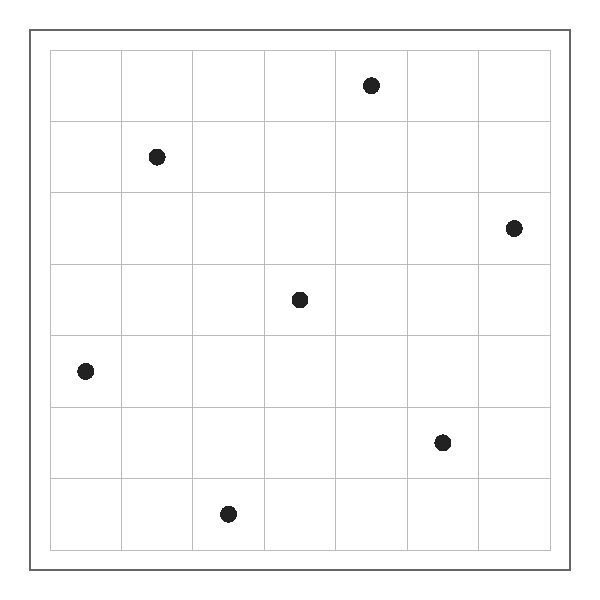
\includegraphics[width=0.33\textwidth]{../figures/1}
\caption{Maximin Latin hypercube sampling design}
\end{figure}

\end{frame}

\note{Let us lay the theoretical foundation. We estimate bold x through Bayes' formula, with a prior and a posterior. At the prior stage we know nothing about the function, so the initial points must cover the space as uniformly as possible. To ensure that in every one-dimensional projection all coordinates are distinct, Morris and Mitchell proposed the maximin Latin hypercube sampling design in 1995; as Figure 1 shows, it covers the space uniformly.}

\begin{frame}{Maximum Projection Design}

Maximum projection design (Joseph et al., 2015)\cite{Joseph2015}: let $D=\left\{\boldsymbol{x}_1,\dots,\boldsymbol{x}_n\right\}$ be a design with $n$ points on $\left[0,1\right]^p$, whose criterion is

\begin{equation}
\min_D\sum_{i=1}^{n}\prod_{j\neq i}\frac{1}{\sum_{k=1}^p\left(x_{ik}-x_{jk}\right)^2}
\tag{1}
\end{equation}

\end{frame}

\note{However, it projects poorly in high dimensions. Joseph et al. therefore proposed the maximum projection design in 2015: for a design bold x 1 to bold x n on the p-dimensional unit interval, the criterion is (1). Since the denominator cannot be zero, distinct coordinates are guaranteed automatically, satisfying the maximin constraint.}

\begin{frame}{Maximum Projection Design}

\begin{figure}
\centering
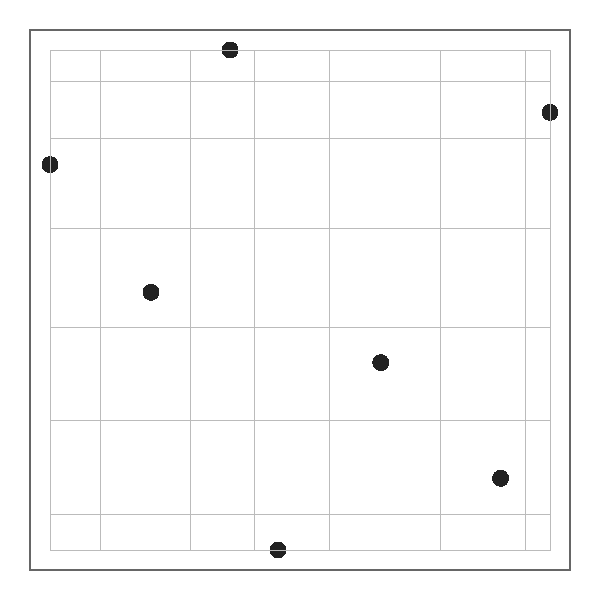
\includegraphics[width=0.33\textwidth]{../figures/2}
\caption{Maximum projection design}
\end{figure}

\end{frame}

\note{As Figure 2 shows, its low-dimensional projections are also uniform. We therefore adopt maximum projection for choosing the initial points.}

\begin{frame}{Maximum OFAT Design with Projection}

Estimator of the total Sobol' index $V_i^\mathrm{tot}$ (Jansen, 1999)\cite{Jansen1999}:

\begin{equation}
\widehat{V_i^{\text{tot}}}=\frac{1}{2m}\left\|h\left(\boldsymbol{A}\right)-h\left(\boldsymbol{A}^{\left(\boldsymbol{B}_i\right)}\right)\right\|^2
\tag{2}
\end{equation}

where $\boldsymbol{A}^{\left(\boldsymbol{B}_i\right)}$ is the matrix obtained by replacing the $i$-th column of the $m\times p$ matrix $\boldsymbol{A}$ with the $i$-th column of $\boldsymbol{B}$, $\left\|\cdot\right\|$ is the Euclidean norm, and $h\left(\boldsymbol{x}\right)$ is an arbitrary function to be tested.

Expectation of the total Sobol' index $V_i^\mathrm{tot}$:

\begin{equation}
\mathrm{E}\left(\widehat{V_i^{\mathrm{tot}}}\right)=\frac{\tau^{2}\sqrt{w_{i}}}{2m}\sum_{j=1}^{m}\left|\boldsymbol{A}_{ji}-\boldsymbol{A}_{ji}^{\left(i\right)}\right|
\tag{3}
\end{equation}

\end{frame}

\note{Ranking factors by importance lets us drop the unimportant ones — fewer factors, easier fitting. The importance of factor i is the total Sobol' index V i total, estimated by Jansen in 1999 as in (2). Since the estimator is random, we examine its expectation, giving (3).}


\begin{frame}{Maximum OFAT Design with Projection}

Criterion for maximizing the total Sobol' index $V_i^\mathrm{tot}$:

\begin{equation}
\argmax_{\boldsymbol{A}}\sum_{j=1}^{m}\left|\boldsymbol{A}_{ji}-\boldsymbol{A}_{ji}^{\left(i\right)}\right|
\tag{4}
\end{equation}

Equation (4) is called the \alert{maximum one-factor-at-a-time design}.

\end{frame}

\note{Because tau times the square root of omega i is constant for fixed i, maximizing (3) reduces to maximizing the L 1 distance, achieved through (4); this is the maximum one-factor-at-a-time design.}

\begin{frame}{Maximum OFAT Design with Projection}

Projection mapping:

\begin{equation}
x_i\leftarrow\begin{cases}x_i-\frac{0.25}{m},&x_i<0.5\\
x_i+\frac{0.25}{m},&x_i\ge0.5\\
x_i,&\text{otherwise}\end{cases},\quad
x_i\leftarrow\begin{cases}x_i+\frac{0.25}{m},&x_i<0.5\\
x_i-\frac{0.25}{m},&x_i\ge0.5\\
x_i,&\text{otherwise}\end{cases}
\tag{5}
\end{equation}

Applying (4) after the mapping in (5) gives the \alert{maximum one-factor-at-a-time design with projection}.

\end{frame}

\note{Inspired by maximum projection, Joseph in 2026 proposed letting bold A and bold B alternately apply the mapping in (5) to improve the projection properties; the two branches in (5) are interchangeable. The result is the maximum one-factor-at-a-time design with projection.}

\begin{frame}{Maximum OFAT Design with Projection}

\begin{figure}
\centering
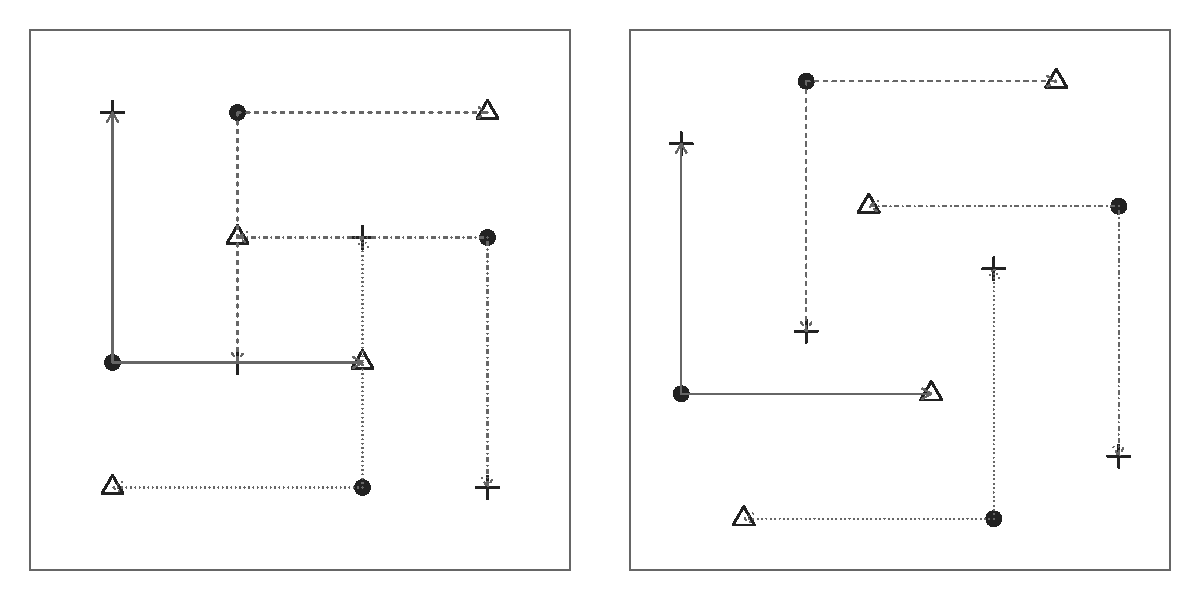
\includegraphics[width=0.50\textwidth]{../figures/3}
\caption{Maximum one-factor-at-a-time design (left) and maximum one-factor-at-a-time design with projection (right)}
\end{figure}

\end{frame}

\note{Figure 3 compares it with the version without projection — the mapped points no longer duplicate coordinates.}

\begin{frame}{Sequential Design}

Sequential design: let $\mathcal{X}\subset\mathbb{R}^p$ be the design space; first choose $x_1\in\mathcal{X}$, then add $x_2,\dots,x_n$ one by one as follows (Joseph, 2016)\cite{Joseph2016}:

\begin{equation}
\boldsymbol{x}_{k+1}=\argmin_{\boldsymbol{x}\in\mathcal{X}}\sum_{i=1}^k\frac{1}{\prod_{j=1}^p\left(x_j-x_{ij}\right)^2}
\tag{6}
\end{equation}

where $k=1,\dots,n-1$.

\end{frame}

\note{We do not need to spend the whole high-fidelity budget at once. We can build a small initial design, collect data, and then decide where the next experiments go. This flexible strategy is the sequential design, also called active learning in machine learning; unlike the maximin Latin hypercube design, the maximum projection design supports it naturally. Define calligraphic X as the design space in the p-dimensional space of blackboard bold R. Joseph proposed in 2016 choosing x 1 as the initial point, then adding x 2 to x n one by one via (6), with k from 1 to n minus 1. In fact, (6) is just the maximum projection criterion (1) rewritten iteratively. We will use it for sequential point selection.}

\begin{frame}{Nested Design}

Suppose there are $K$ fidelity levels, where ``1'' denotes the lowest fidelity and ``$K$'' the highest fidelity, and the corresponding sets of design points are $\left\{D_i\right\}_{i=1}^K$.

Fusion formula (Kennedy and O'Hagan, 2000)\cite{KennedyOHagan2000}:

\begin{equation}
h_k\left(\boldsymbol{x}\right)=h_{k-1}\left(\boldsymbol{x}\right)+\delta_k\left(\boldsymbol{x}\right)
\tag{7}
\end{equation}

where $k=2,\dots,K$, and $\delta_k\left(\boldsymbol{x}\right)$ denotes the bias between the outputs of the $(k-1)$-th and the $k$-th fidelity levels. We make the following Gaussian process assumptions:

\begin{equation}
\begin{aligned}
&\delta_k\left(\boldsymbol{x}\right)\sim\mathcal{GP}\left\{0,\tau_k^2R_k\left(\cdot\right)\right\}\\
&h_\mathrm{L}\left(\boldsymbol{x}\right)\sim\mathcal{GP}\left\{\mu,\tau_\mathrm{L}^2R_\mathrm{L}\left(\cdot\right)\right\}
\end{aligned}
\tag{8}
\end{equation}

\end{frame}

\note{Suppose there are K fidelity levels, 1 the lowest and K the highest, with design sets D i, i from 1 to K. Kennedy and O'Hagan fused the data as in (7), assuming Gaussian processes as in (8).}

\begin{frame}{Nested Design}

\begin{definition}[Gaussian Process]
If for arbitrarily chosen $\boldsymbol{x}_1,\dots,\boldsymbol{x}_n$ and any integer $n\ge1$, the vector $\boldsymbol{Y}=\left\{Y\left(\boldsymbol{x}_1\right),\dots,Y\left(\boldsymbol{x}_n\right)\right\}'$ follows a multivariate normal distribution, then the random function $Y\left(\boldsymbol{x}\right)$ is called a Gaussian process.
\end{definition}

\end{frame}

\note{Recall: a Gaussian process is a random function whose values at any finite set of points follow a multivariate normal distribution — a generalization of the multivariate normal to arbitrary dimensions.}

\begin{frame}{Nested Design}

Nested design (Kennedy and O'Hagan, 2000): \alert{$D_1\supset D_2\supset\dots\supset D_K$}.

Sequential maximum-entropy (Shannon, 1948)\cite{Shannon1948} design problem:

\begin{equation}
\begin{aligned}D_1^*&=\argmax_{D_1}\left|\boldsymbol{R}_1\left(D_1,D_1\right)\right|\\
D_2^*&=\argmax_{D_2\subseteq D_1^*}\left|\boldsymbol{R}_2\left(D_2,D_2\right)\right|\end{aligned}
\tag{9}
\end{equation}

where $\left|\cdot\right|$ is the determinant, and $\boldsymbol{R}_k\left(D,D'\right)$ is the correlation matrix of the $k$-th fidelity level whose $\left(i,j\right)$ element is $R_k\left(\boldsymbol{a}_i-\boldsymbol{b}_j\right)$.

\end{frame}

\note{They also proposed a nested design: D 1 contains D 2, and so on down to D K. Consider the two maximum-entropy design problems in (9). Entropy, defined by Shannon in 1948, measures uncertainty; experimental design seeks larger entropy, i.e., more information — exactly what maximum projection maximizes, making it ideal for D 1 star and D 2 star.}

\begin{frame}{Nested Design}

The optimal sample point to remove from $D_1$ is (Joseph, 2026)\cite{Joseph2026}:

\begin{equation}
x^*_k=\argmax_{x_k\in D_1}\sum_{j\neq k}\frac{1}{\prod_{l=1}^{p}\left\{\left|x_{kl}-x_{jl}\right|+\beta_{l}\right\}^{2}}
\tag{10}
\end{equation}

\begin{figure}
\centering
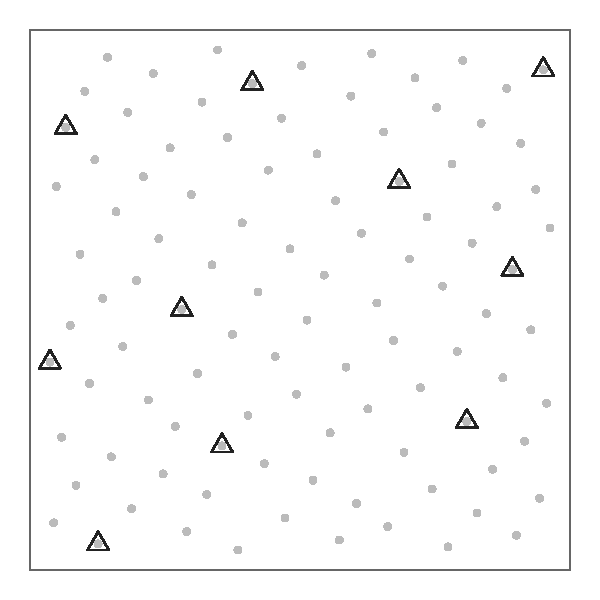
\includegraphics[width=0.33\textwidth]{../figures/4}
\caption{Nested design with two fidelity levels}
\end{figure}

\end{frame}

\note{Joseph in 2026 noted that the nested design is built by successively removing points from D 1 star to form D 2 star, with the removal criterion in (10). Unlike (6), the denominator adds a positive constant beta l, because D 2 takes discrete values from the continuous D 1: two points coincide with probability zero in a continuous space, but not in a discrete one, so the constant prevents a zero denominator. Figure 4 shows the nested design with two fidelity levels: the triangular D 2 points are discrete points chosen from the circular D 1 points, both following maximum projection.}

\begin{frame}{Expected Improvement Method}

Optimization objective of the black-box function:

\begin{equation}
\min_{\boldsymbol{x}\in\left[0,1\right]^p}h\left(\boldsymbol{x}\right)
\tag{11}
\end{equation}

Iterative formula for finding the next design point:

\begin{equation}
\boldsymbol{x}_{n+1}=\argmin_{\boldsymbol{x}}\widehat{h_n}\left(\boldsymbol{x}\right)
\tag{12}
\end{equation}

This procedure is repeated until convergence. Since the Gaussian process adopts a Bayesian framework, such problems are called \alert{Bayesian optimization methods}. Expected improvement method (Jones et al., 1998)\cite{Jones1998}: let the experimental design be $D_n=\left\{\boldsymbol{x}_1,\dots,\boldsymbol{x}_n\right\}$, with observed data $\boldsymbol{y}_n=\left(y_1,\dots,y_n\right)'$. 

\end{frame}

\note{Now to the core optimization problem: minimize the expensive black-box function h bold x over the design space, taken as the p-dimensional unit interval, giving (11) — a nonlinear problem with box constraints. We need a global method using as few evaluations as possible. We select a small design bold x 1 to bold x n, evaluate h bold x i to get y i, and approximate the function by a cheap Gaussian process surrogate hat h n bold x, which approaches the high-fidelity surface sequentially. Minimizing the surrogate yields the next point via (12); iterating until convergence gives Bayesian optimization. The standard choice is expected improvement, proposed by Jones et al. in 1998. }

\begin{frame}{Expected Improvement Method}

Place a Gaussian process prior on the unknown function:

\begin{equation}
h\left(\boldsymbol{x}\right)\sim\mathcal{GP}\left\{\mu,\tau^2R\left(\cdot\right)\right\}
\tag{13}
\end{equation}

where $\mu$ is the constant mean, $\tau^2$ the variance, and $R\left(\cdot\right)$ the correlation function. Let $\boldsymbol{R}_n$ be the $n\times n$ correlation matrix whose $\left(i,j\right)$ element is $R\left(\boldsymbol{x}_i-\boldsymbol{x}_j\right)$, $\boldsymbol{r}_n\left(\boldsymbol{x}\right)$ the correlation vector whose $i$-th element is $R\left(\boldsymbol{x}-\boldsymbol{x}_i\right)$, and $\boldsymbol{1}_n$ the $n$-dimensional column vector of all ones.

\end{frame}

\note{Given the design D n and observations bold y n, we place the Gaussian process prior (13).}

\begin{frame}{Expected Improvement Method}

Its posterior distribution (Joseph, 2026, Lemma 2.2):

\begin{equation}
\begin{aligned}
h\left(\boldsymbol{x}\right)\mid D_n,\boldsymbol{y}_n
&\sim\mathcal{N}\Bigl\{\mu+\boldsymbol{r}_n\left(\boldsymbol{x}\right)'\boldsymbol{R}_n^{-1}\left(\boldsymbol{y}_n-\mu\boldsymbol{1}_n\right),\\
&\qquad\tau^2\left(1-\boldsymbol{r}_n\left\{\boldsymbol{x}\right\}'\boldsymbol{R}_n^{-1}\boldsymbol{r}_n\left\{\boldsymbol{x}\right\}\right)\Bigr\}
\end{aligned}
\tag{14}
\end{equation}

Let $h_{\mathrm{min}}^{\left(n\right)}=\min \boldsymbol{y}_n$, and define the improvement function:

\begin{equation}
I\left(\boldsymbol{x}\right)=\max\left\{h_{\mathrm{min}}^{\left(n\right)}-h\left(\boldsymbol{x}\right),0\right\}
\tag{15}
\end{equation}

Thus, if the chosen $x$ satisfies $h\left(\boldsymbol{x}\right)<h_{\mathrm{min}}^{\left(n\right)}$, an \alert{improvement is obtained}; otherwise there is no improvement.

\end{frame}

\note{By Lemma 2.2 of Joseph in 2026, the posterior is (14). Let h n minimum be the minimum of bold y n and define the improvement I in (15): improvement occurs when h bold x falls below h n minimum.}

\begin{frame}{Expected Improvement Method}

Iterative formula for expected improvement:

\begin{equation}
\boldsymbol{x}_{n+1}=\argmax_{\boldsymbol{x}}\mathrm{E}\left\{I\left(\boldsymbol{x}\right)\mid D_n,\boldsymbol{y}_n\right\}
\tag{16}
\end{equation}

Explicit expression of expected improvement (Jones et al., 1998):

\begin{equation}
\boldsymbol{x}_{n+1}=\argmax_{\boldsymbol{x}}\left\{s_n\left(\boldsymbol{x}\right)\left[u_n\left\{\boldsymbol{x}\right\}\Phi\left(u_n\left\{\boldsymbol{x}\right\}\right)+\phi\left(u_n\left\{\boldsymbol{x}\right\}\right)\right]\right\}
\tag{17}
\end{equation}

where $\phi\left(\cdot\right)$ and $\Phi\left(\cdot\right)$ denote the standard normal probability density function and the standard normal cumulative distribution function, respectively; $s_n\left(\boldsymbol{x}\right)$ is the posterior standard deviation, and $u_n\left\{\boldsymbol{x}\right\}=\left\{h_{\mathrm{min}}^{\left(n\right)}-\widehat{h_n}\left(\boldsymbol{x}\right)\right\}/s_n\left(\boldsymbol{x}\right)$. 

\end{frame}

\note{Since I is random, we maximize its expectation, giving the iterative rule (16). Jones et al. derived its explicit form (17).}

\begin{frame}{Expected Improvement Method}

Derivatives of the explicit expression:

\begin{equation}
\frac{\partial\mathrm{EI}}{\partial\widehat{h_n}\left(\boldsymbol{x}\right)}=-\Phi\left\{u_n\left\{\boldsymbol{x}\right\}\right\}<0,\quad\frac{\partial\mathrm{EI}}{\partial s_n\left(\boldsymbol{x}\right)}=\phi\left\{u_n\left\{\boldsymbol{x}\right\}\right\}>0
\tag{18}
\end{equation}

where $\mathrm{EI}=s_n\left(\boldsymbol{x}\right)\left[u_n\left\{\boldsymbol{x}\right\}\Phi\left(u_n\left\{\boldsymbol{x}\right\}\right)+\phi\left(u_n\left\{\boldsymbol{x}\right\}\right)\right]$

\end{frame}

\note{And differentiating yields (18): expected improvement decreases with hat h n bold x and increases with s n bold x, balancing optimization against surrogate accuracy.}

\begin{frame}{Expected Improvement Method}

\begin{figure}
\centering
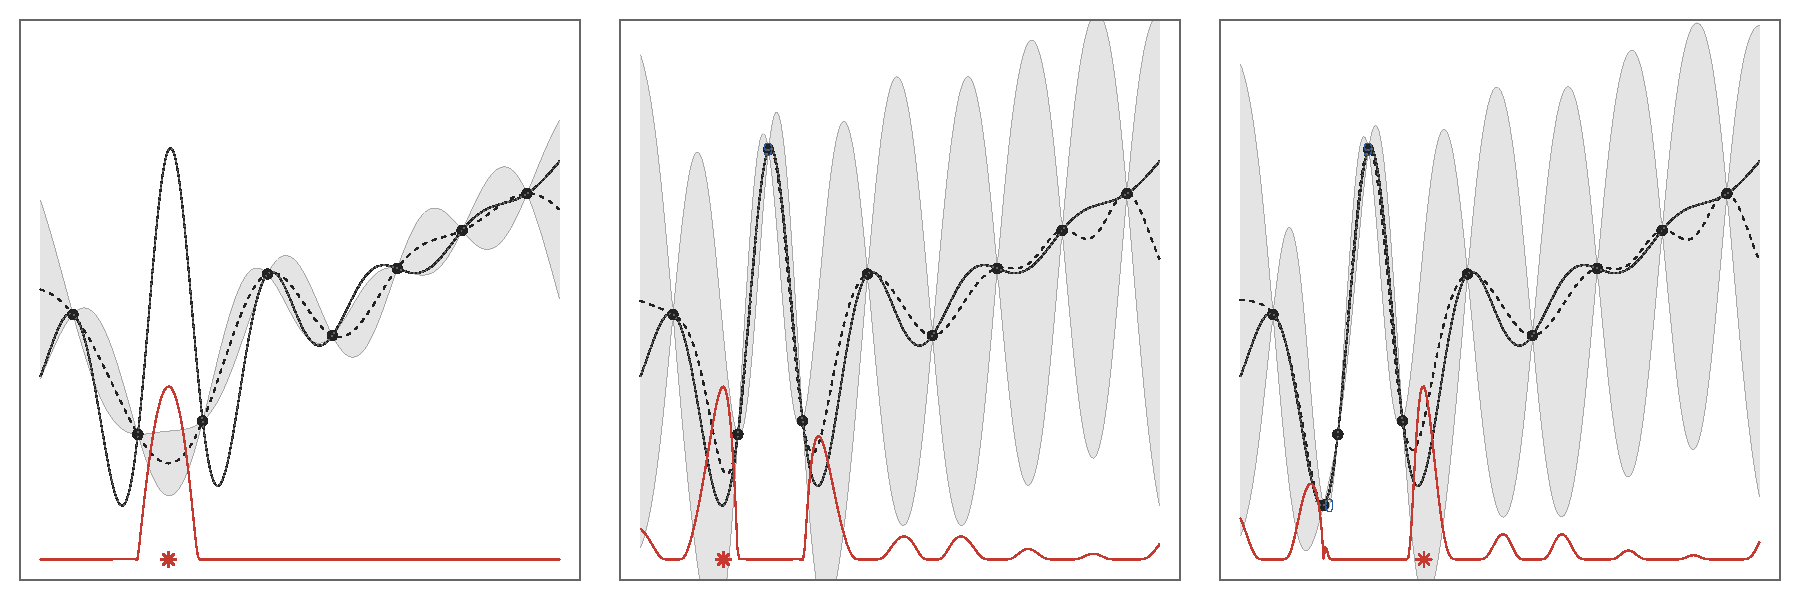
\includegraphics[width=0.98\textwidth]{../figures/5}
\caption{Two iterations of the expected improvement minimization algorithm on a test function}
\end{figure}

\end{frame}

\note{Figure 5 shows two iterations on a test function, gradually locating its minimum and second minimum.}

\begin{frame}{Test Functions}

One-dimensional test function (Joseph, 2026):

\begin{equation}
h\left(x\right)=\frac{\sin\left(10\pi x\right)}{1+64\left(x-0.25\right)^2}+x^2
\tag{19}
\end{equation}

where $x\in\left[0,1\right]$.

Two-dimensional Branin function (Surjanovic and Bingham, 2013)\cite{SurjanovicBingham2013}:

\begin{equation}
f\left(\boldsymbol{x}\right)=\left(x_2-\frac{5.1}{4\pi^2}x_1^2+\frac{5}{\pi}x_1-6\right)^2+10\left(1-\frac{1}{8\pi}\right)\cos x_1+10
\tag{20}
\end{equation}

where $x_1\in\left[-5,10\right]$ and $x_2\in\left[0,15\right]$.

\end{frame}

\note{We now pick test functions of 1, 2, 4, and 8 dimensions to compare the pipeline across dimensions. These are: the one-dimensional test function of Joseph in 2026, it's in (19); the Branin function of Surjanovic and Bingham in 2013, it's in (20);}

\begin{frame}{Test Functions}

Simple additive function (Joseph, 2026):

\begin{equation}
h\left(\boldsymbol{x}\right)=\sum_{k=1}^{4}\frac{1}{k}\sin\left(\left\{k^2+1\right\}\pi x_k\right)
\tag{21}
\end{equation}

where $\boldsymbol{x}\in\left[0,1\right]^4$.

Function simulating borehole water flow (Morris et al., 1993)\cite{Morris1993}:

\begin{equation}
y=\frac{2\pi x_3\left(x_4-x_6\right)}{\log\left(\frac{x_2}{x_1}\right)\left\{1+\frac{2x_7x_3}{\log\left(x_2/x_1\right)x_1^2x_8}+\frac{x_3}{x_5}\right\}}
\tag{22}
\end{equation}

where $x_1\in\left[0.05,0.15\right]$, $x_2\in\left[100,50000\right]$, $x_3\in\left[63070,115600\right]$, $x_4\in\left[990,1110\right]$, $x_5\in\left[63.1,116\right]$, $x_6\in\left[700,820\right]$, $x_7\in\left[1120,1680\right]$, $x_8\in\left[9855,12045\right]$.

\end{frame}

\note{a four-factor additive function of Joseph in 2026, it's in (21); and the borehole water flow function of Morris et al. in 1993, it's in (22).}

\begin{frame}{Multi-Fidelity}

General formula for constructing multi-fidelity functions (Song et al., 2024)\cite{Sung2024}:

\begin{equation}
f_\mathrm{L}\left(\boldsymbol{x}\right)=f_\mathrm{H}\left(\boldsymbol{x}\right)+\frac cp\cdot\sum_{i=1}^p\left(x_i-\frac12\right)
\tag{23}
\end{equation}

\end{frame}

\note{For each test function we construct a low-fidelity version. Inspired by Song et al. in 2024, I use the general form (23): the high-fidelity function plus a constant c times the average shift from 0.5, with c set to 10 to 15 percent of the range of f H.}

\begin{frame}{Multi-Fidelity}

Low-fidelity versions of the four test functions:

\begin{align*}
f_\mathrm{L}\left(x\right)&=f_\mathrm{H}\left(x\right)+0.3\left(x-\frac{1}{2}\right)
\tag{24}\\
f_\mathrm{L}\left(\boldsymbol{u}\right)&=f_\mathrm{H}\left(\boldsymbol{u}\right)+40\cdot\frac{u_1+u_2-1}{2}
\tag{25}\\
f_\mathrm{L}\left(\boldsymbol{x}\right)&=f_\mathrm{H}\left(\boldsymbol{x}\right)+0.5\cdot\frac{\sum_{k=1}^{4}\left(x_k-\frac{1}{2}\right)}{4}
\tag{26}\\
f_\mathrm{L}\left(\boldsymbol{u}\right)&=f_\mathrm{H}\left(\boldsymbol{u}\right)+70\cdot\frac{\sum_{i=1}^{8}\left(u_i-\frac{1}{2}\right)}{8}
\tag{27}\\
\end{align*}

\end{frame}

\note{The resulting low-fidelity versions are given in (24) to (27).}

\section{Complete Pipeline}

\begin{frame}{Complete Pipeline}

Complete pipeline M1:

\begin{equation}
\begin{aligned}
&\quad\;\;\boxed{\text{Maximum Projection Design}}\to\boxed{\text{Sequential Design}}\\
&\to\boxed{\text{Nested Design}}\to\boxed{\text{Expected Improvement}}
\end{aligned}
\tag{28}
\end{equation}

Blank control M0:

\begin{equation}
\boxed{\text{Maximum Projection Design}}\to\boxed{\text{Expected Improvement}}
\tag{29}
\end{equation}

\end{frame}

\note{Now the experiments. The complete pipeline is M1 in (28); the blank control M0 in (29) drops both the sequential and nested designs.}

\begin{frame}{Complete Pipeline}

Removing only the nested design S1:

\begin{equation}
\begin{aligned}
&\quad\;\;\boxed{\text{Maximum Projection Design}}\to\boxed{\text{Sequential Design}}\\
&\to\boxed{\text{Expected Improvement}}
\end{aligned}
\tag{30}
\end{equation}

Removing only the sequential design S2:

\begin{equation}
\begin{aligned}
&\;\;\quad\boxed{\text{Maximum Projection Design}}\to\boxed{\text{Nested Design}}\\
&\to\boxed{\text{Expected Improvement}}
\end{aligned}
\tag{31}
\end{equation}

\end{frame}

\note{To attribute each component's contribution, we also build S1, removing only the nested design (30), and S2, removing only the sequential design (31).}

\begin{frame}[fragile]{Calibration Experiment}

\textbf{Output 1}: optimal number of high-fidelity evaluations for each dimension

\begin{verbatim}
n2* by dimension: d1=2   d2=14   d4=14   d8=14
\end{verbatim}

Following the M1 workflow, the room for the sequential and fusion components is \alert{squeezed out almost entirely by the budget}.

\end{frame}

\note{The calibration experiment fixes the budget split. We sweep the initial number of high-fidelity evaluations from 2 to 15; the value 1 is unsolvable, since a single point cannot fit a Gaussian process. For each setting we run M1 twenty times, record f star once the budget is exhausted, and take the median as the metric, choosing the n star with the smallest median. Output 1 shows the optimum: 2 for dimension 1, and 14 for dimensions 2, 4, and 8. Low-dimensional functions are easy to fit; the difficulty explodes in high dimensions. And since the optima for 2, 4, and 8 dimensions sit on the grid endpoint 14, under the tiny budget of 15 high-fidelity equivalents the initial design dominates — the sequential and fusion components have almost no room left.}

\begin{frame}[fragile]{Ablation Experiment}

\textbf{Output 2}: table of function minima fitted by the four experimental configurations in each of the four dimensions after forcing 5 high-fidelity evaluations

\begin{verbatim}
  config         d1          d2          d4         d8
      M1 -0.6035453   3.1626952   -1.410891   19.68542
      S2 -0.6035453   0.4041193   -1.606024   12.70143
      S1  0.0000000   5.4693989   -1.187530   17.15853
      M0  0.0000000   0.8787899   -1.297524   10.50205
M0@n2=14 -0.5776889   2.2567621   -1.448456   12.59210
\end{verbatim}

\end{frame}

\note{The ablation experiment identifies each component's marginal contribution while controlling the initial design. Using n 2 star directly would leave too few low-fidelity samples, degenerate the pipeline into pure high fidelity, and make the four configurations indistinguishable. So we force exactly 5 high-fidelity evaluations per dimension, repeat twenty times, and obtain Output 2.}

\begin{frame}[fragile]{Ablation Experiment}

\begin{verbatim}
  config         d1          d2          d4         d8
      M1 -0.6035453   3.1626952   -1.410891   19.68542
      S2 -0.6035453   0.4041193   -1.606024   12.70143
      S1  0.0000000   5.4693989   -1.187530   17.15853
      M0  0.0000000   0.8787899   -1.297524   10.50205
M0@n2=14 -0.5776889   2.2567621   -1.448456   12.59210
\end{verbatim}

\begin{itemize}
\item In the 1-dimensional case, the expected improvement method \alert{fails}.
\item In the 4-dimensional case, the fusion model uses a \alert{large amount of low-fidelity data} to correct the approximation of the high-fidelity surface.
\item The screening component provides \alert{no positive contribution} in any of the four dimensions: the bias structure between low and high fidelity makes the factor importance ranking unreliable.
\end{itemize}

\end{frame}

\begin{frame}[fragile]{Ablation Experiment}

\begin{verbatim}
  config         d1          d2          d4         d8
      M1 -0.6035453   3.1626952   -1.410891   19.68542
      S2 -0.6035453   0.4041193   -1.606024   12.70143
      S1  0.0000000   5.4693989   -1.187530   17.15853
      M0  0.0000000   0.8787899   -1.297524   10.50205
M0@n2=14 -0.5776889   2.2567621   -1.448456   12.59210
\end{verbatim}

\begin{itemize}
\item The value of fusion decays as the dimension increases: in the 8-dimensional case, the blank control is actually better than the fusion-only configuration, which is a manifestation of the \alert{curse of dimensionality} within the multi-fidelity framework.
\item Under the same budget, a few high-fidelity points combined with fusion \alert{far outperform} running with many high-fidelity points alone.
\end{itemize}

\end{frame}

\section{Summary}

\begin{frame}{Summary}

\begin{itemize}
\item Under an extremely small budget, the initial design \alert{dominates the results}; the room for the sequential and fusion components is squeezed out almost entirely by the budget.
\item Fusion is the \alert{decisive component}: in low dimensions, it goes from failure to the global optimum; in high dimensions, it is constrained by the curse of dimensionality.
\item The screening component provides \alert{no positive contribution}: the bias structure between low and high fidelity makes the factor importance ranking unreliable.
\item Under the same budget, a few high-fidelity points combined with fusion \alert{far outperform} running with many high-fidelity points alone.
\end{itemize}

\end{frame}

\section{Future Work}

\begin{frame}{Future Work}

Direction for improvement: under what bound on the total Sobol' index of the bias field $\delta\left(\boldsymbol{x}\right)$ does the factor importance ranking given by the low-fidelity function preserve the true high-fidelity ranking?

\end{frame}

\begin{frame}[fragile]{Github}
All the above codes, figures and tex source files have been uploaded to

\begin{verbatim}
https://github.com/wenje-ma/singapore
\end{verbatim}

Everyone is welcome to reproduce the results.
\end{frame}

\begin{frame}[standout]

Thank you for listening!

\end{frame}

\begin{frame}[allowframebreaks]{References}

\printbibliography

\end{frame}

\end{document}
